\documentclass[12pt]{article}
\usepackage[english]{babel}
\usepackage[utf8]{inputenc}

%% Pointer to 'default' preamble, other reusable files
% pacakages and definitions

\usepackage{geometry}
\geometry{
	letterpaper, 
	portrait, 
	top=.75in,
	left=.8in,
	right=.75in,
	bottom=.5in		} 	% Page Margins
	
%% additional packages for nice things
\usepackage{amsmath} 	% for most math
\usepackage{commath} 	% for abs
\usepackage{lastpage}	% for page count
\usepackage{amssymb} 	% for therefore
\usepackage{graphicx} 	% for image handling
\usepackage{wrapfig} 	% wrap figures
\usepackage[none]{hyphenat} % for no hyphenations
\usepackage{array} 		% for >{} column characterisctis
\usepackage{physics} 	% for easier derivative \dv....
\usepackage{tikz} 		% for graphic@!
\usepackage{circuitikz} % for circuits!
\usetikzlibrary{arrows.meta} % for loads
\usepackage[thicklines]{cancel}	% for cancels
\usepackage{xcolor}		% for color cancels
\usepackage[per-mode=fraction]{siunitx} % for si units and num
\sisetup{group-separator = {,}, group-minimum-digits = 3} % additional si unit table functionality

\usepackage{fancyhdr} 	% for header
\usepackage{comment}	% for ability to comment out large sections
\usepackage{multicol}	% for multiple columns using multicols
\usepackage[framed,numbered]{matlab-prettifier} % matlab sytle listing
\usepackage{marvosym} 	% for boltsymbol lightning
\usepackage{pdflscape} 	% for various landscape pages in portrait docs.
%\usepackage{float}
\usepackage{fancyvrb}	% for Verbatim (a tab respecting verbatim)
\usepackage{enumitem}	% for [resume] functionality of enumerate
\usepackage{spreadtab} 	% for using formulas in tables}
\usepackage{numprint}	% for number format in spread tab
\usepackage{subcaption} % for subfigures with captions
\usepackage[normalem]{ulem} % for strike through sout

% for row colors in tables....
\usepackage{color, colortbl}
\definecolor{G1}{gray}{0.9}
\definecolor{G2}{rgb}{1,0.88,1}%{gray}{0.6}
\definecolor{G3}{rgb}{0.88,1,1}

% For table formatting
\usepackage{booktabs}
\renewcommand{\arraystretch}{1.2}
\usepackage{floatrow}
\floatsetup[table]{capposition=top} % put table captions on top of tables

% Caption formating footnotesize ~ 10 pt in a 12 pt document
\usepackage[font={small}]{caption}

%% package config 
\sisetup{output-exponent-marker=\ensuremath{\mathrm{E}}} % for engineer E
\renewcommand{\CancelColor}{\color{red}}	% for color cancels
\lstset{aboveskip=2pt,belowskip=2pt} % for more compact table
%\arraycolsep=1.4pt\def
\setlength{\parindent}{0cm} % Remove indentation from paragraphs
\setlength{\columnsep}{0.5cm}
\lstset{
	style      = Matlab-editor,
	basicstyle = \ttfamily\footnotesize, % if you want to use Courier - not really used?
}
\renewcommand*{\pd}[3][]{\ensuremath{\dfrac{\partial^{#1} #2}{\partial #3}}} % for larger pd fracs
\renewcommand{\real}[1]{\mathbb{R}\left\{ #1 \right\}}	% for REAL symbol
\newcommand{\imag}[1]{\mathbb{I}\left\{ #1 \right\}}	% for IMAG symbol
\definecolor{m}{rgb}{1,0,1}	% for MATLAB matching magenta
	
%% custom macros
\newcommand\numberthis{\addtocounter{equation}{1}\tag{\theequation}} % for simple \numberthis command

\newcommand{\equal}{=} % so circuitikz can have an = in the labels
\newcolumntype{L}[1]{>{\raggedright\let\newline\\\arraybackslash\hspace{0pt}}m{#1}}
\newcolumntype{C}[1]{>{\centering\let\newline\\\arraybackslash\hspace{0pt}}m{#1}}
\newcolumntype{R}[1]{>{\raggedleft\let\newline\\\arraybackslash\hspace{0pt}}m{#1}}

%% Header
\pagestyle{fancy} % for header stuffs
\fancyhf{}
% spacing
\headheight 29 pt
\headsep 6 pt
%%% custom commands for nicer units
\newcommand{\mw}{\ensuremath{\text{ MW}}}
\newcommand{\hz}{\ensuremath{\text{ Hz}}}
\newcommand{\pu}{\ensuremath{\text{ Pu}}}
\newcommand{\sbase}{\ensuremath{\text{S}_{\text{Base}}}}
\newcommand{\fbase}{\ensuremath{f_{\text{Base}}}}
\newcommand{\mbase}[1]{\ensuremath{\text{M}_{\text{Base}_{#1}}}}
\newcommand{\hsys}{\ensuremath{\text{ H}_{\text{sys}}}}


%% Header
\rhead{Thad Haines \\ Page \thepage\ of \pageref{LastPage}}
\chead{DTC Results of undesirable BPA Governor Response \\ 02-24-20}
\lhead{Research \\ }

%\usepackage{graphicx}
%\graphicspath{ {figures/} }
%\newcommand{\caseName}{ }

\begin{document}
\paragraph{Initial Definite Time Controller (DTC) BPA Result Summary} \ \\
Using a six machine system, results show that the method of stepping Pref while also gaining input $\Delta\omega_{PU}$ produces similar generator output action provided by BPA as an 'undesirable' response.
Remaining differences believed to be caused by differences in model size, time constants, and actual 'feed-forward' action.

% results...
%\begin{minipage}{.49\linewidth}
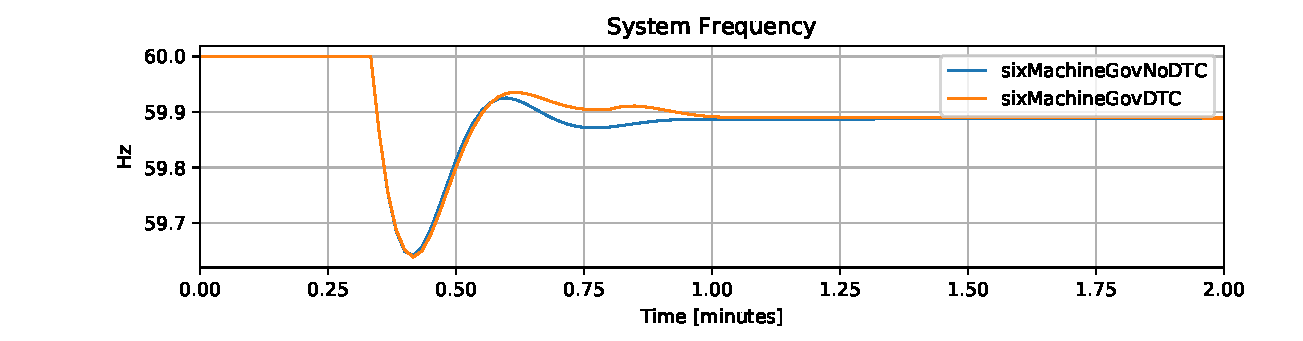
\includegraphics[width=\linewidth]{figures/f}
%\end{minipage}%
%\begin{minipage}{.49\linewidth}
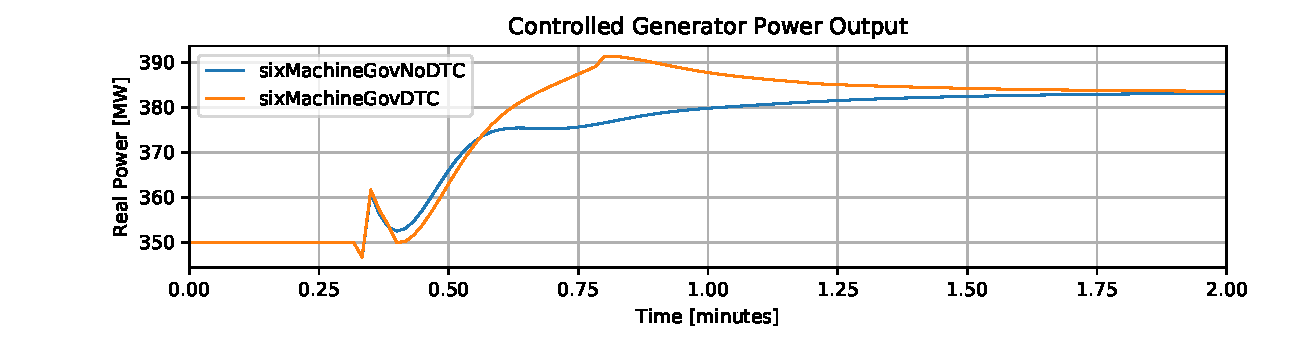
\includegraphics[width=\linewidth]{figures/pe}
%\end{minipage}

%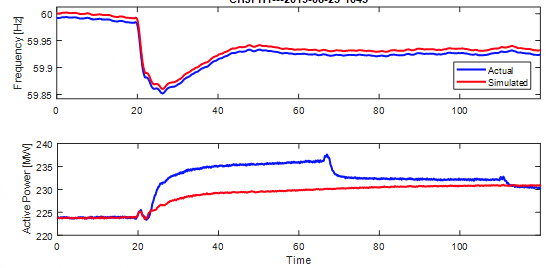
\includegraphics[width=.8\linewidth]{figures/givenData}


\paragraph{Modified Governor Model} \ \\
Input $\omega$ block moved so that gain would be more logical.

%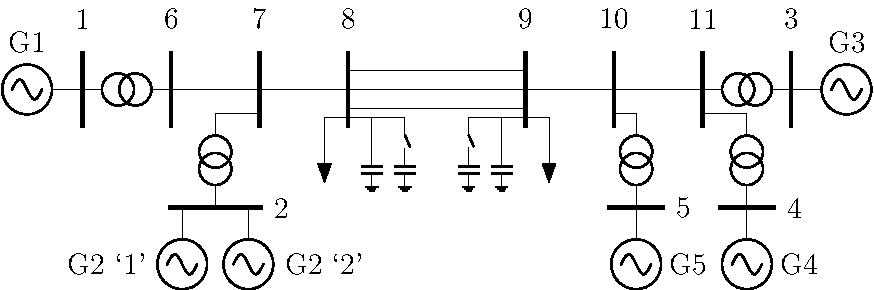
\includegraphics[width=\linewidth]{../../models/sixMachine/sixMachine}
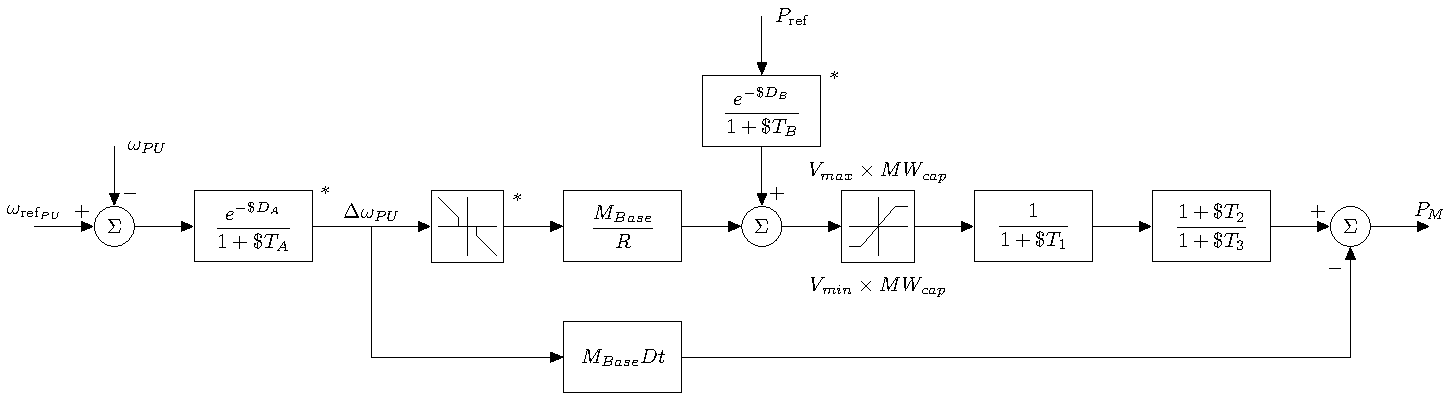
\includegraphics[width=\linewidth]{../../models/tgov1/tgov1DBdelay}

\pagebreak
\paragraph{Code Example and Explanation}
Code used to define system step, governor delay, and DTC action is provided below.
In practice, this code is user defined in the simulation .ltd.py file.\\
\vspace{1em}

An ungoverned generator on bus 5 has mechanical power stepped down 100 MW at t=20 to simulate the tripping of a generator.
A governor delay block is used to gain the $\omega$ input by $0.5$.
DTC action occurs every 24 seconds (so that first action is near frequency nadir) and sets  $P_{ref} = P_{ref0} + \dfrac{\Delta \omega}{R}M_{base} * 0.5 $.\\

\vspace{1em}

\begin{lstlisting}[language=Python]
# Perturbances
mirror.sysPerturbances = [
    'gen 5 : step Pm 20 -100 rel', # Step no-gov generator down
    ]

# Delay block used as delta_w gain
mirror.govDelay ={
    'delaygen2' : {
        'genBus' : 2,
        'genId' : '1', # optional
        'wDelay' : (0, 0, .5),
        'PrefDelay' : (0, 0)
        },
    #end of defined governor delays
    }

# Definite Time Controller Definitions
mirror.DTCdict = {
    'bpaTest' : {
        'RefAgents' : {
            'ra1' : 'mirror : f',
            'ra2' : 'gen 2 1 : R', 
            'ra3' : 'gen 2 1 : Pref0',
            'ra4' : 'gen 2 1 : Mbase',
            },# end Referenc Agents
        'TarAgents' : {
            'tar1' : 'gen 2 1 : Pref',
            }, # end Target Agents
        'Timers' : {
            'set' :{ # set Pref
                'logic' : "(ra1 > 0)", # should always eval as true
                'actTime' : 24, # seconds of true logic before act
                'act' : "tar1 = ra3 + (1-ra1)/(ra2) * ra4 *0.5 ", # step Pref 
            },# end set
            'reset' :{ # not used in example
                'logic' : "0",
                'actTime' : 0, # seconds of true logic before act
                'act' : "0", # set any target On target = 0
            },# end reset
            'hold' : 0, # minimum time between actions (not used in example)
            }, # end timers
        },# end bpaTest
    }# end DTCdict

\end{lstlisting}

\end{document}